\section{\acl{pdms}} \label{sec:pdms}

Das \acf{pdms} unterstützt die klinische Dokumentation auf Intensivstationen \glqq\acf{icu}\grqq{} und hat damit nachweisbare Auswirkungen auf die Vollständigkeit der Patientenakten, den Zeitaufwand für die Dokumentation und die Erhöhung der Patientenqualitätssicherung \cite{pdmsfinanc, pdmsimplem, pdmsicu}. Dieses System umfasst auch Komponenten der computergestützten Auftragserfassung für Ärzte \glqq\ac{cpoe}\grqq{}, denn die Daten aus diesem System sind entscheidend für verschiedene automatisierte Workflows \cite{pdmsfinanc, pdmsicu}. Das \ac{pdms} bietet auch eine spezifische Funktionalität für die Dokumentation der \ac{drg}, welche alle relevanten Daten für die Codierung erfasst \cite{pdmsfinanc, pdmsimplem}.

In Deutschland waren im Jahr 2021 ca. 15 \ac{pdms}-Anbieter bekannt \cite{pdmsgermany}. Unter diesen Anbietern befindet sich der \acf{copra}, welcher an der Universitätsmedizin Mainz und Standort der Realisierung dieses Projekts benutzte \ac{pdms} ist.

\subsection{\acsu{copra}}

\acs{copra} System GmbH ist seit 1993 einer der führenden Anbieter von \acp{pdms} in Deutschland \cite{copradosing, copra}. Dessen Hauptprodukt ist das zertifizierte Medizinprodukt \ac{copra} in der Version 6 \glqq\ac{copra}6\grqq{}. Mit seinen vier Anwendungsgebieten: Ärzte und Ärztinnen, Pflege, Controlling und \ac{it}-Abteilung ist \ac{copra} ein \ac{pdms} für die Dokumentation von Behandlung und Pflege geeignet \cite{copra}. Aus diesem Grund wird \ac{copra} als \ac{pdms} seit 2007 an der Universitätsmedizin Mainz etabliert \cite{copraplaces}.

Für die Ärzte und Ärztinnen bietet das \ac{copra}-System eine transparente und vereinfachte Möglichkeit für die Dokumentation aller relevanten Daten einer Behandlung, denn alle Befunde der behandelnden Personen können in \ac{copra} eingesehen werden, darüber hinaus werden ärztliche Anordnungen dokumentiert und freigeschaltet \cite{copra}.

Mit den sogenannten Arbeitslisten für die Pflege werden die bereits erfolgten und nicht erfolgten Behandlungsschritte in \ac{copra} angezeigt. Außerdem werden die Kurven der Vitalparameter durch die automatische Übernahme von Werten aller an Patienten angeschlossenen Geräte aufgezeichnet. \cite{copra}.

Die Dokumentation der gesammelten Aktivitäten in \ac{copra} werden exportiert, sodass Therapieverfahren und Maßnahmen durch das Controlling ermittelt werden \cite{copra}.

\ac{copra} nutzt etablierte \ac{it}-Technologien, wie Microsoft \acs{sql} Server und .NET Framework, ist skalierbar, virtualisierbar und bietet Freiheiten bei der Gestaltung der Infrastruktur, sodass es für die \ac{it}-Abteilungen attraktiv ist \cite{copra}.

Durch die Freiheiten bei der Gestaltung der Infrastruktur von \ac{copra} ist ein multidimensionales Datenmodell wie in der \ref{fig:copraschema} möglich. 

Das Schema der \ref{fig:copraschema} stellt nur das Datenmodell des Bereichs für die Durchführung dieses Projekts dar, denn das \ac{copra}-System beinhaltet ein Schema mit mehr als 260 Tabellen insgesamt im Release 44.0 der Version 1 von 20.10.2015 \cite{copradoc}. Dieses Modell sollte aber nicht mit einem Sternschema in einem \ac{dw} (\ref{subsec:datamodel}) verwechselt werden, denn bei \ac{copra} stellt die Tabelle \texttt{co6\_medic\_data\_patient} mit den Basisinformationen der behandelnden Personen, in der \ac{dw}-Theorie (\ref{sec:dw}), eine Dimension dar, und die weiteren Tabellen sammeln Metadaten und die Ergebnisse der Messungen der medizinischen Geräte (Werttabellen), also die Fakten, und beinhalten auch die Hauptschlüssel von \texttt{co6\_medic\_data\_patient} als Fremdschlüssel.

\clearpage

\begin{figure}[ht]
	\centering
	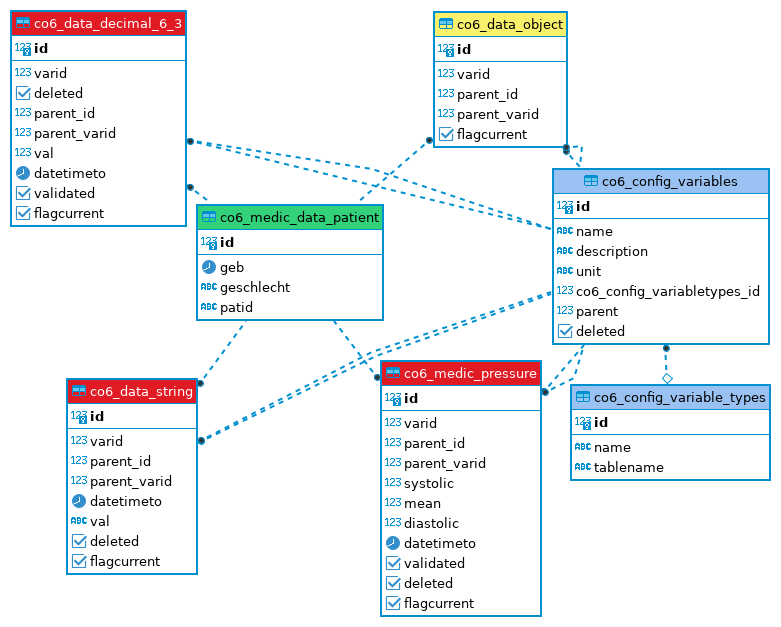
\includegraphics[height=8.5cm]{figures/copra_data_model_data}
	\caption[Datenmodell von \acs{copra}]{Datenmodell des für diese Arbeit benutzten Teils vom \ac{copra}-System an der Universitätsmedizin Mainz. Die Tabelle \texttt{co6\_medic\_data\_patient} beinhaltet die Informationen der behandelnden Personen. Die Tabellen \texttt{co6\_data\_decimal\_6\_3}, \texttt{co6\_medic\_data\_pressure} und \texttt{co6\_data\_string} speichern die Ergebnisse der Messungen oder Techniken. Die Tabelle \texttt{co6\_data\_object} beinhaltet die Schlüssel aller Objekte, z. B. Patienten und abstrakte Elemente, wie die Arztbriefe oder Scores.
	Die Tabellen \texttt{co6\_config\_variables} und \texttt{co6\_config\_variable\_types} beinhalten die Metadaten der gespeicherten Informationen in \ac{copra}.}
	\label{fig:copraschema}
\end{figure}

Der Teil der \ac{copra}-\ac{db} ist zugleich eine der Datenquelle im Staging Bereich des \ac{dw}  im \ac{diz} an der Universitätsmedizin Mainz (\ref{fig:dizummz}).